% comparaison de p sur la methode de permutation aleatoire
%% ---- pas encore REPROGRAMMER -- utiliser la fonction de cout unitaire
\begin{figure}[htb!] 
\centering
% meilleur probabilite p parmi les [0.0, 0.1, 0.2, ...., 1.0]
% a changer par des chemins relatifs
%\includegraphics[scale=0.25]{permut_aleatoire_coutMin_degreMin_fct_cout_normal_500G/aleatoire/courbes/comparaison_probabilities_p_00_10_moy_dh_aleatoire_p_10.jpeg}
\includegraphics[scale=0.25]{comparaison_probabilities_p_00_10_moy_dh_aleatoire_p_10.jpeg}
\caption{ Comparaison des diff\'erentes probabilit\'es d'ajout $k \in [1,9]$ de corr\'elations fausses positives et fausses n\'egatives sur la m\'ethode de permutation al\'eatoire }
\label{compareDifferentesProbabilitesP0_1_fct_cout_unitaire_p05} 
\end{figure}
%% ---- pas encore REPROGRAMMER

Faisons varier la variable $p\_correl \in [0,1]$ par pas de $0.1$ dans le but de visualiser l'impact de corr\'elations {\em fausses positives} et {\em fausses n\'egatives} dans l'ex\'ecution des algorithmes. Rappelons que l'ajout et la suppression d'ar\^etes ont le m\^eme co\^ut de traitement c'est-\`a-dire $1$.
La figure \ref{compareDifferentesProbabilitesP0_1_fct_cout_unitaire_p05} r\'esume l'\'evolution des types d'erreurs de corr\'elations ($p\_correl$) pour des distances de Hamming $moy\_DH$ en fonction de  $k \in [1, 9]$  erreurs de corr\'elations.
\newline 
Nous constatons que les algorithmes donnent de meilleurs r\'esultats pour $p\_correl = 1$ et de mauvais r\'esultats pour $p\_correl = 0$. 
En d'autres termes, lorsqu'on ajoute que des corr\'elations {\em fausses n\'egatives} i.e $p\_correl  = 1$ dans la matrice $matE$, les algorithmes  proposent, dans la majorit\'e des cas, un line graphe $LG_k$ dont ces erreurs de corr\'elation sont supprim\'ees. Cela s'illustre dans la figure \ref{permut_distanceMoyenDLDH_k_5_9_aleatoire_p_10} o\`u l'ajout de $5$ corr\'elations {\em fausses n\'egatives} influencent tr\`es peu les line graphes propos\'es $LG_{k}$ puisqu'ils sont identiques aux line graphes initiales $LG$ dans $45\%$ des cas. 
En revanche, ce pourcentage baisse avec beaucoup d'erreurs de corr\'elations. Tel est le cas pour $k = 9$ corr\'elations o\`u le taux est de $24\%$. 
\begin{figure}[htb!] 
\centering
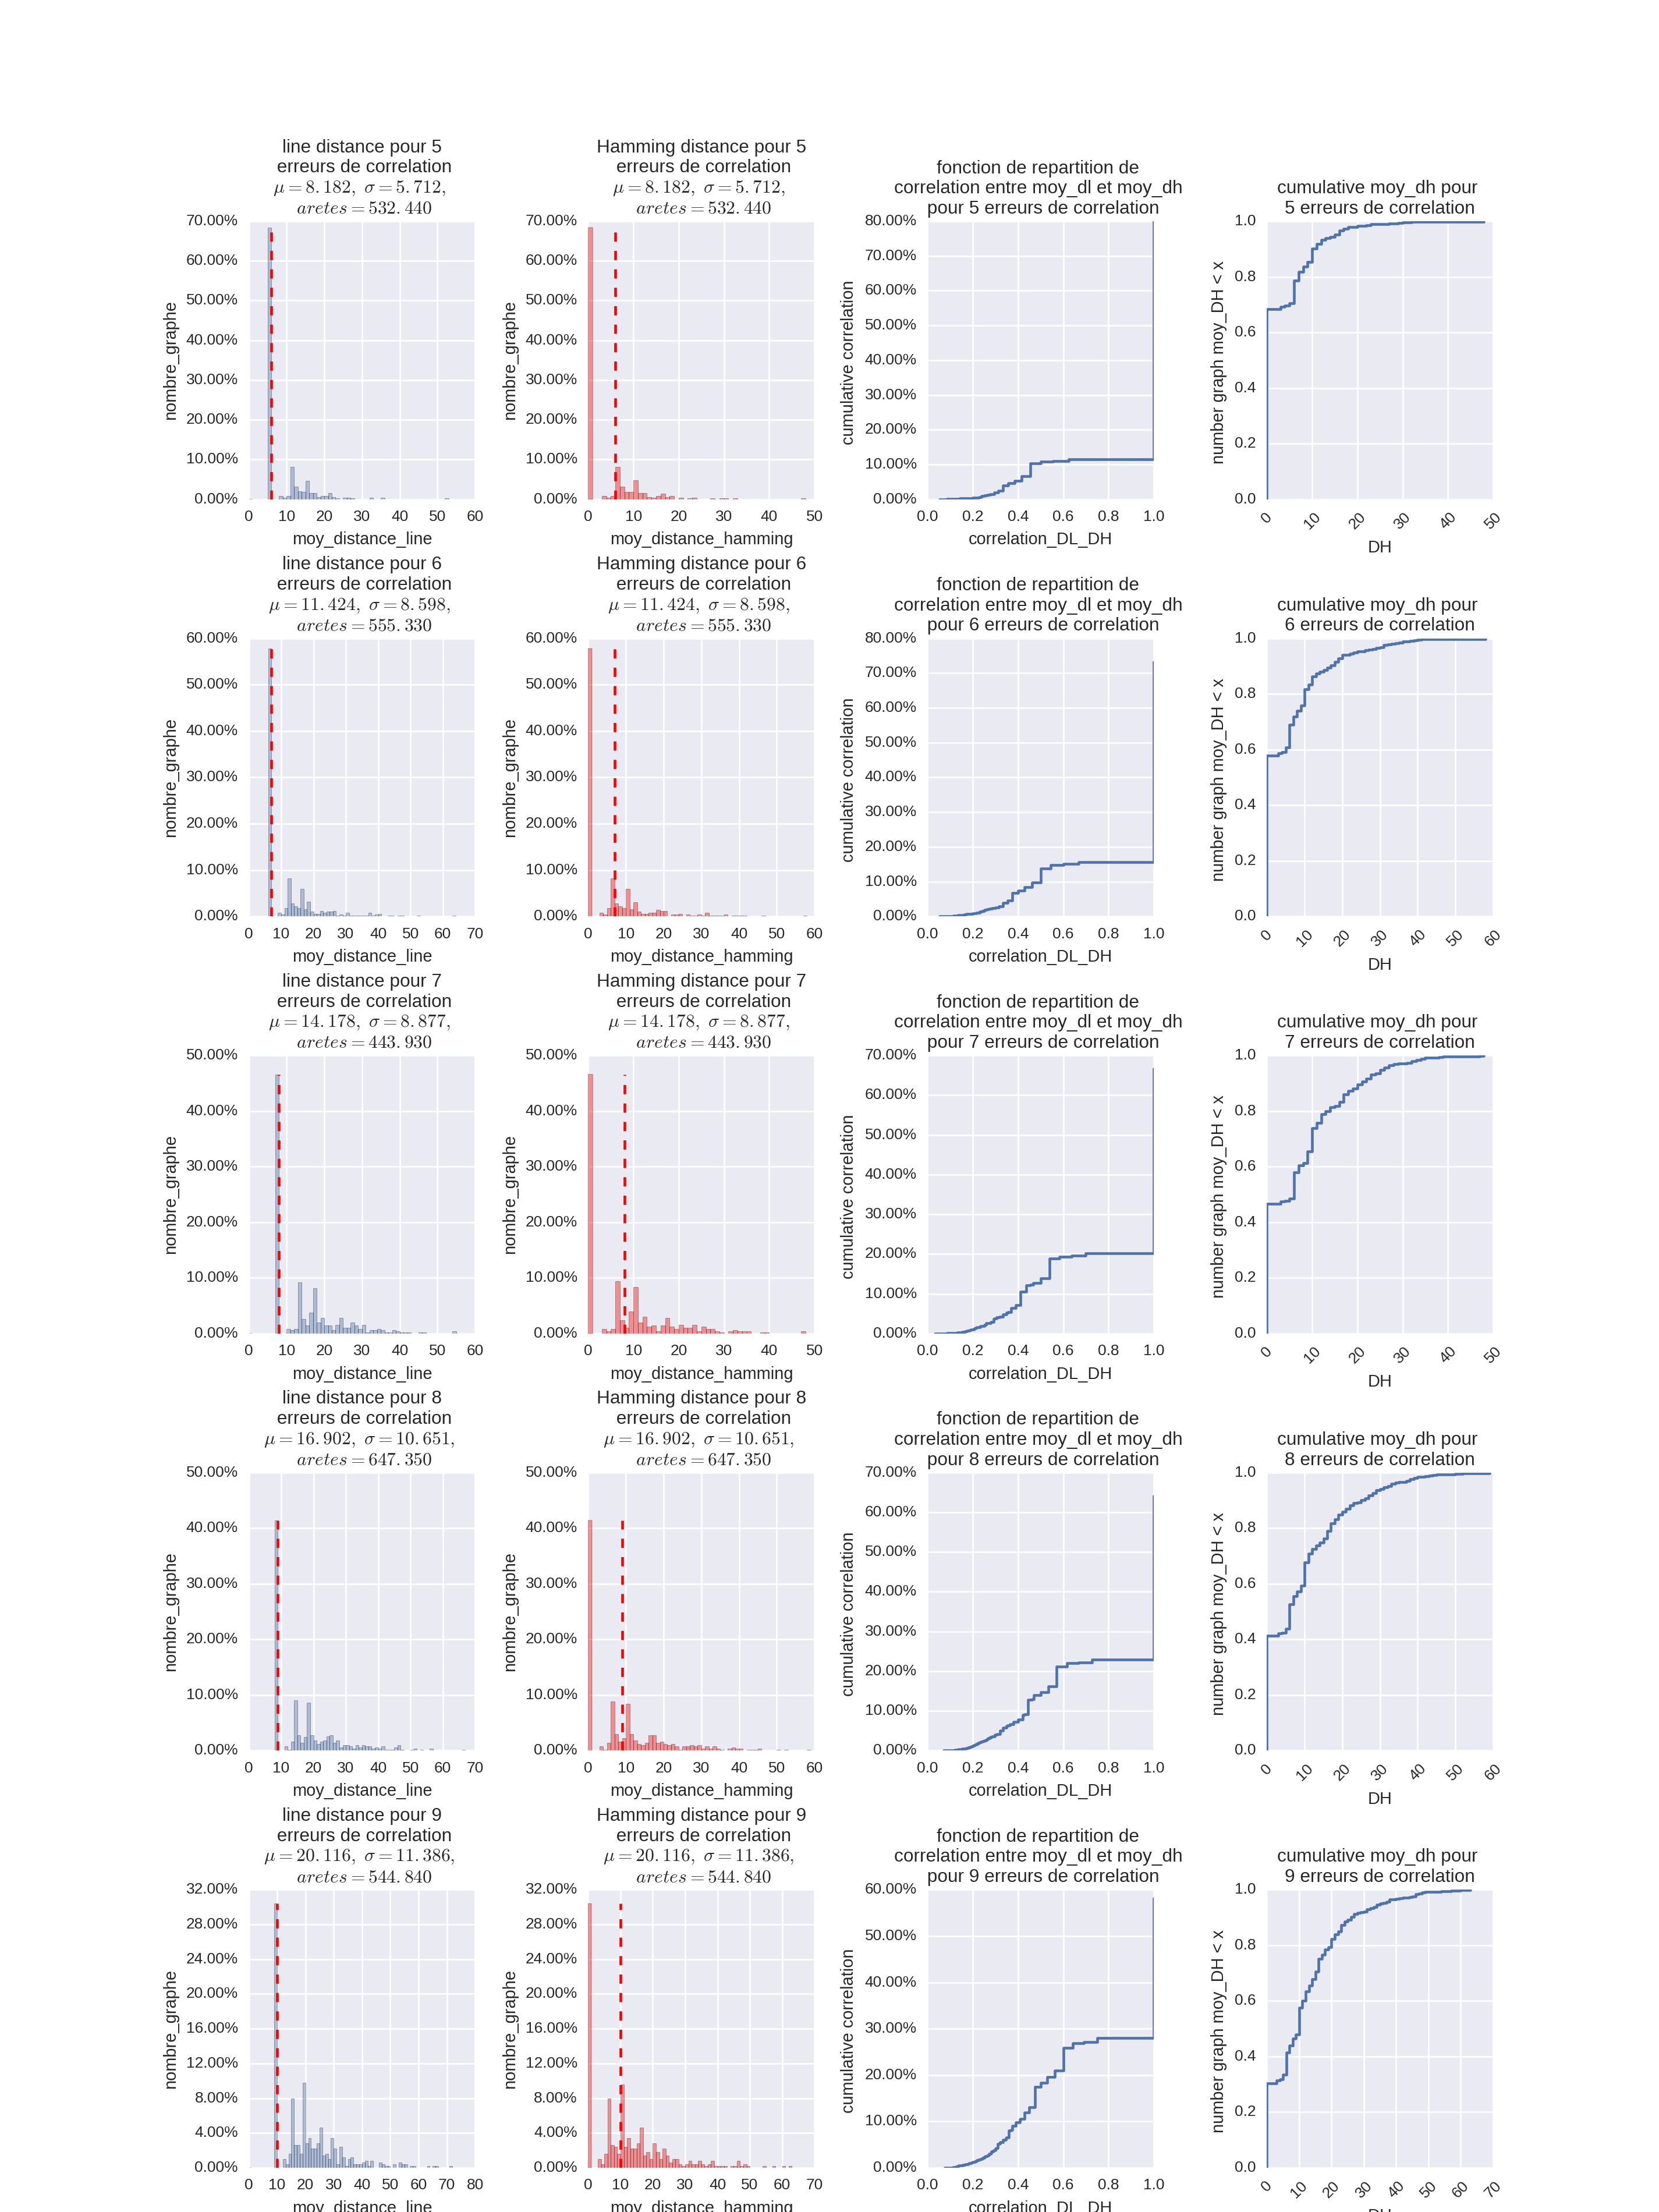
\includegraphics[width=550pt,height=600pt]{permut_distanceMoyenDLDH_k_5_9_aleatoire_p_10.jpeg}
\caption{ M\'ethode de permutation al\'eatoire avec une fonction de correction \`a co\^ut unitaire et $p\_correl = 1.0$ : distribution des distances line $moy\_DL$ et de Hamming $moy\_DH$ pour $k \in [6,  9]$ corr\'elations alter\'ees}
\label{permut_distanceMoyenDLDH_k_5_9_aleatoire_p_10} 
\end{figure}
%En revanche, ce pourcentage baisse malgr\'e le nombre \'elev\'e de corr\'elations {\em fausses positives}. Tel est le cas pour $k = 9$ corr\'elations o\`u le taux est de $24\%$. 
\newline
Par ailleurs, le mauvais r\'esultat obtenu pour des probabilit\'es $p\_correl < 0.5$ s'explique par le mode de fonctionnement de l'algorithme de correction. En Effet, cet algorithme consiste \`a ajouter des ar\^etes au voisinage du sommet \`a corriger puis de supprimer certaines ar\^etes pour \'eviter qu'un sommet n'appartienne \`a plus de $2$ cliques (propriet\'e du line graphe).
\newline
Nous pensons que le meilleur compromis est la probabilit\'e $p\_correl = 0.7$ parce que, pour peu de corr\'elations modifi\'ees ($k<5$), les lines graphes produits $LG_k$ et g\'en\'er\'es $LG$ diff\`erent de $k<6$ ar\^etes correspondant aux $k$ erreurs de  corr\'elations \'effectu\'ees  et au d\'el\`a $k \geq 6$, le nombre d'ar\^etes diff\'erentes est fonction du nombre de corr\'elations faites multipl\'e par $1.5$.
Cela signifie qu'il faut, dans la matrice de corr\'elation, $30\%$ de corr\'elations {\em fausses positives} et $70\%$ de corr\'elation {\em fausses n\'egatives}. 
\newline
%Que se passe-t-il si on priorise l'ajout de corr\'elations {\em fausses n\'egatives} \`a chaque traitement c'est-\`a-dire la suppression d'ar\^etes?  
%En d'autres termes, l'ajout d'ar\^etes {\em fausses positives} a un co\^ut moins important que celui des {\em fausses n\'egatives}. 
%----
Que se passe-t-il si on priorise l'ajout de corr\'elations {\em fausses positives} \`a chaque traitement c'est-\`a-dire l'ajout d'ar\^etes?  
En d'autres termes, la suppression d'ar\^etes {\em fausses n\'egatives} a un co\^ut moins important que celui des {\em fausses positives}. 
%----